\documentclass[a4paper,german]{article}
%Mainly taken from
%https://github.com/gillescastel/university-setup/blob/master/preamble.tex
%but edited for own purposes

%%%%%OWN
%%Own basic packages
\usepackage{mkessler-math}
\usepackage{mkessler-fancythm}
\usepackage{mkessler-operators}

\usepackage{datetime}
\date{{\normalfont Mitschrift}\\{\sc Maximilian Keßler}}

\usepackage{wrapfig}
\usepackage{pgfplots}
\pgfplotsset{compat=1.7}
%%%%%%Preamble from Gilles Castel
% Some basic packages
\usepackage{url}
\usepackage{graphicx}
\usepackage{float}

% for wrapping text around figures
\usepackage{wrapfig}

%%This option is for now commented out, not sure what it does, but causes errors
%\pdfminorversion=7


% Don't indent paragraphs, leave some space between them
\usepackage{parskip}

% Hide page number when page is empty
\usepackage{emptypage}
% Other font I sometimes use.
\usepackage{xcolor}
% \usepackage{cmbright}

% Math stuff
\usepackage{amsfonts}

% Put x \to \infty below \lim
\let\svlim\lim\def\lim{\svlim\limits}

%Make implies and impliedby shorter
\let\implies\Rightarrow
\let\impliedby\Leftarrow
\let\iff\Leftrightarrow
\let\epsilon\varepsilon

% Command for short corrections
% Usage: 1+1=\correct{3}{2}

% Environments
\makeatother

% Fix some spacing
% http://tex.stackexchange.com/questions/22119/how-can-i-change-the-spacing-before-theorems-with-amsthm
\makeatletter
\def\thm@space@setup{%
  \thm@preskip=\parskip \thm@postskip=0pt
}


% \lecture starts a new lecture (les in dutch)
%
% Usage:
% \lecture{1}{di 12 feb 2019 16:00}{Inleiding}
%
% This adds a section heading with the number / title of the lecture and a
% margin paragraph with the date.

% I use \dateparts here to hide the year (2019). This way, I can easily parse
% the date of each lecture unambiguously while still having a human-friendly
% short format printed to the pdf.

\usepackage{xifthen}
\def\testdateparts#1{\dateparts#1\relax}
\def\dateparts#1 #2 #3 #4 #5\relax{
    \marginpar{\small\textsf{\mbox{#1 #2 #3 #5}}}
}

\def\@lecture{}%
\newcommand{\lecture}[3]{
    \ifthenelse{\isempty{#3}}{%
    \def\@lecture{\ifenglish Lecture\else Vorlesung\fi\, #1}%
    }{%
\def\@lecture{\ifenglish Lecture\else Vorlesung\fi\, #1: #3}%
    }%
    \subsection*{\@lecture}
    \marginpar{\small\textsf{\mbox{#2}}}
}

% These are the fancy headers
\usepackage{fancyhdr}
\pagestyle{fancy}

% LE: left even
% RO: right odd
% CE, CO: center even, center odd
% My name for when I print my lecture notes to use for an open book exam.
% \fancyhead[LE,RO]{Gilles Castel}

\fancyhead[RO,LE]{\@lecture} % Right odd,  Left even
\fancyhead[RE,LO]{}          % Right even, Left odd

\fancyfoot[RO,LE]{\thepage}  % Right odd,  Left even
\fancyfoot[RE,LO]{}          % Right even, Left odd
\fancyfoot[C]{\leftmark}     % Center

\makeatother

% Todonotes and inline notes in fancy boxes
\usepackage{todonotes}

% Make boxes breakable
\tcbuselibrary{breakable}

% Figure support as explained in my blog post.
\usepackage{import}
\usepackage{xifthen}
\usepackage{pdfpages}
\usepackage{transparent}
\newcommand{\incfig}[1]{%
    \def\svgwidth{\columnwidth}
    \import{./figures/}{#1.pdf_tex}
}

% Fix some stuff
% %http://tex.stackexchange.com/questions/76273/multiple-pdfs-with-page-group-included-in-a-single-page-warning
\pdfsuppresswarningpagegroup=1






\title{{Einführung in die} \\ Geometrie und Topologie}
\author{{\normalfont Dozent}\\{\sc Dr. Daniel Kasprowski}}

\renewcommand\subset\subseteq
%\DeclareMathOperator{\Topo}{O}
\def\Topo{\mathcal{O}}

\begin{document}
    \maketitle
    \section{testing}
    ref : \ref{thm:heine-borel}, \\
nameref:    \nameref{thm:heine-borel}\\
autoref: \autoref{thm:heine-borel} \\
cref: \cref{thm:heine-borel} \\
ref: \ref{thm:point-in-hausdorff-space-is-closed} \\
autoref:    \autoref{thm:point-in-hausdorff-space-is-closed} \\
cref:    \cref{thm:point-in-hausdorff-space-is-closed} \\
nameref:    \nameref{thm:point-in-hausdorff-space-is-closed} \\
\listoftheorems
    \tableofcontents
    % start lectures
    \lecture[Motivationsfragen. Brown'sche Bewegung. Ereignisse, Wahrscheinlichkeiten, Modell von Zufallsexperimenten.]{Mo 12 Apr 2021 10:16}{Grundbegriffe}

\begin{itemize}
    \item Es gibt ein Helpdesk, auch explizit für Studentinnen
    \item die Vorlesung wird aufgenommen, und zwar ohne Videos der Teilnehmenden sowie des Dozenten, die Aufzeichnung werden anschließend in Sciebo hochgeladen.
    \item Es gibt ein Diskussionsforum für Fragen (auf eCampus).
    \item Ab heute Abend, 18 Uhr (Mo 12 Apr 2021 18:00), kann man sich auf eCampus für die Übungsgruppen registrieren und endet am Dienstag Abend um 24 Uhr (Di 12 Apr 2021 24:00), es wird versucht, die Studenten gleichmäßig zu verteilen.
    \item Falls ihr in der Warteliste landet und gewünscht ist, in der Gruppe abzugeben, schreibt eine Mail mit den gewünschten Abgabepartner, dann kann eine gemeinse Einteilung erfolgen.
    \item Es gibt auch das Modul \verb?AlmaIIb?. Registriert euch noch nicht, dies ist für den 2. Teil der Vorlesung notwendig. 
    \item Die Abgabe der Übungsblätter erfolgt einheitlich jeden Freitag um 12 Uhr.
    \item Gruppenabgaben sind erlaubt, bis zu einer Größe von maximal 4 StudentInnen.
    \item Das 1. Blatt ist freiwillig und gibt Bonuspunkte.
    \item Für die Klausurzulassung werden 50\% der Punkte benötigt. Von den Programmieraufgaben müssen mindestens 4 von 6 zufriedenstellend bearbeitet werden.
    \item Programmieraufgaben gibt es ab dem 2. Übungsblatt auf jedem 2. Blatt. Die Bearbeitungszeit beträgt dann 2 Wochen.
\end{itemize}


\section*{Einleitung}
In der Vorlesung werden wir sehen:
\begin{description}
    \item[Teil 1: Diskrete Stochastik]
        \begin{itemize}
            \item Zufallsvariablen
            \item Bedingte Wahrscheinlichkeiten
            \item Unabhängigkeit von Variablen
            \item Monte-Carlo Methoden
        \end{itemize}
    \item[Teil 2: Numerische Analysis]
        \begin{itemize}
            \item Iterative Verfahren
            \item Interpolation von Daten (durch Polynome, trigonometrische Funktionen, \ldots)
            \item Numerische Verfahren für die Integration
        \end{itemize}
\end{description}


\section{Diskrete Stochastik}
\subsection{Einleitung}
\begin{goal}
    Beschreibung von Systemen, die einen Anteil an \vocab{Zufall} haben, d.h. nicht 100\% deterministisch sind.
\end{goal}
\begin{example}
    \begin{itemize}
        \item Spiele: Kartenspiele, Glücksspiele, \ldots
        \item Statistik: Umfragen, Versicherung
        \item Komplexe Systeme: Wettermodelle, Finanzmärkte
    \end{itemize}
\end{example}

\underline{Was sind Quellen von Zufall?}
\begin{itemize}
    \item Zu komplexe Systeme. Dann sieht der Gesamteffekt zufällig aus.
    \item Fehlende Informationen (z.B. bei einem Kartenspiel)
    \item Chaotische Systeme (Wetter
    \item Intrinsisch unvorhersagbare Systeme (z.B. radioaktiver Zerfall)
\end{itemize}
\begin{question}
    \begin{enumerate}[(1)]
        \item Wie modelliert man ein System mit Zufall?
        \item Wie simuliert man ein System mit Zufall? (anwendungstechnischer)
        \item Welche Voraussagen kann man machen?
    \end{enumerate}
\end{question}


\begin{example}
    Die \vocab{Brown'sche Bewegung}. Das System ist implizit ein Pollen mit vielen Wassermolekülen ($\sim 10^{23})$, die sich im Prinzip deterministisch bewegen. \\
    $\implies$ Wir erhalten ein Gleichungssystem mit $(N+1)\cdot 6$ (3 Positionen, 3 Geschwindigkeit) Variablen. Dieses ist de facto unlösbar. \\

    Was wollen wir hier eigentlich untersuchen? -> Die Bewegung des Pollens, jedoch nicht die der einzelnen Wassermoleküle. \\
    In einer \vocab{Modellierung} ersetzt man die Stöße, die ,durch die Wassermoleküle entstehen durch \vocab{zufällige Stöße}. 
\end{example}

\underline{Diskretes Modell:} Die Zeit bewegt sich in $n\in \left \{0,1,2,\ldots\right\} $. Sei
\[
    Z(n) := (\text{Position des Pollens zur Zeit $n$}) \in  \Z^3
.\] 
OBdA setzen wir $Z(0) = 0$. \\
\underline{Dynamik}: $Z(n+1) = Z(n) + \xi_n$, wobei wir $\xi_n$ aus dem Ergebnis eines Würfelwurfs bestimmen werden:
 \[
\xi_n = \begin{cases}
    (1,0,0) & \text{wenn Würfel}=1 \\
    (-1,0,0) & \text{wenn Würfel}=2 \\
    (0,1,0) & \text{wenn Würfel}=3 \\
    (0,-1,0) & \text{wenn Würfel}=4 \\
    (0,0,1) & \text{wenn Würfel}=5 \\
    (0,0,-1) & \text{wenn Würfel}=6
\end{cases}
.\] 

\begin{question}
    Welche Fragen können wir mit solch einem System nun beantworten? Was pasiert, wenn $n\gg 1$?
\end{question}
\begin{enumerate}[\protect\circled{\alph*}]
    \item Typischerweise erhalten wir $\abs{Z(n)} =  O(\sqrt{n}) $ 
    \item Wenn wir die Frequenz von $[Z(n)]_i$ betrachten, (d.h. bei welcher Koordinate in Richtung $i$ befinden wir uns nach  $n$ Würfen) sehen wir typischerweise: 
        \begin{figure}[h]
            \centering
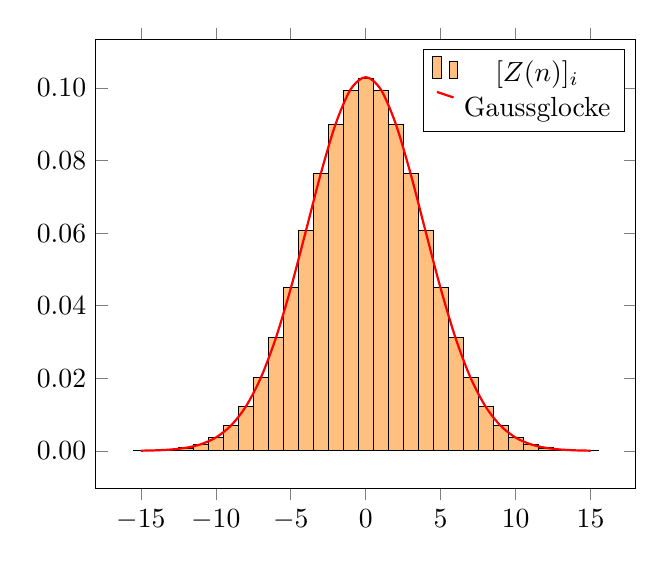
\begin{tikzpicture}[
    declare function={binom(\k,\n,\p)=\n!/(\k!*(\n-\k)!)*\p^\k*(1-\p)^(\n-\k);}
]
\begin{axis}[
    samples at={-15,...,15},
    yticklabel style={
        /pgf/number format/fixed,
        /pgf/number format/fixed zerofill,
        /pgf/number format/precision=2
    },
    ybar=0pt, bar width=1
]
\addplot [fill=orange, fill opacity=0.5] {binom(x+30,60,0.5)}; \addlegendentry{$[Z(n)]_i$}
    \addplot[draw=red,thick,smooth] {1/(sqrt(30*pi)) *exp(-1/30*x^2)}; \addlegendentry{\text{Gaussglocke}}
\end{axis}
\end{tikzpicture}
\caption{Binomialverteilung und Gaussglocke}
\end{figure}
Für $n\gg 1$ sieht diese Verteilung dann ungefähr wie die Gaussglocke aus. \\
\end{enumerate}
\underline{Skalierung:} Wir setzen nun
\[
    B(t) = \lim_{n \to \infty} \frac{Z(\left\lfloor nt \right\rfloor )}{\sqrt{n} }
.\] 
und dies ist dann die Brownsche Bewegung.

Nun möchten wir Vorhersagen treffen können:
\begin{question}
        Ist $Z(n)$ in einer gegebenen Menge  $A$?
\end{question}
Das kann man (im Allgemeinen) nicht einfach mit 'Ja' oder 'Nein' beantworten. Stattdessen müssen wir fragen:
\begin{question}
Wenn man $Z(n)$ beobachtet, wie häufig wird  $Z(n)$ in  $A$ sein?
\end{question}
Diese Frage lässt sich mit einer Zahl $\in [0,1]$ beantworten.

\subsection{Ereignisse und Wahrscheinlichkeiten}
Wir benötigen 3 Grundelemente:
\begin{enumerate}[(1)]
    \item Die Menge $\Omega$ von möglichen \vocab{Ergebnissen}. die Elemente von $\Omega$ heißen auch  \vocab{Elementarereignisse}.
    \item Die Menge $\mathcal{F}$ der \vocab{Ereignisse}. Ein Ereignis  $E$ ist eine Eigenschaft, die mit einer Teilmenge $G\subset \Omega$ assoziiert ist: $ω\in G \iff $ Eigenschaft $E$ ist erfüllt.
    \item Eine \vocab{Wahrscheinlichkeitsverteilung (auch W-maß)}:
        \[
            \mathbb{P}: \mathcal{F} \to  [0,1]
        .\] 
\end{enumerate}
\begin{remark*}
    Wir werden noch sehen, dass gewisse Dinge für unsere Begriffe erfüllt sein müssen, dazu aber später mehr.
\end{remark*}

\begin{example}
    Eine Urne hat 12 nummerierte Kugeln (von 1 bis 12).
    \begin{enumerate}[(1)]
        \item Das \vocab{Zufallsexperiment} besteht daraus, dass wir eine Kugel aus der Urne ziehen und die Zahl notieren, die wir sehen. D.h.
            \[
            \Omega = \left \{1,\ldots,12\right\} 
            .\] 
            Ein Elementarereignis ist nun z.B. gegeben durch $ω = \left \{5\right\}  \equiv 5$ (wir vereinfachen die Notation).
        \item Mögliche Ereignisse sind z.B:
            \begin{equation}
                \begin{split}
                    A &= \text{'Die Zahl ist gerade'} \\
                    B&= \text{'Die Zahl ist }\leq 5 \text{'}\\
                    C &= \text{'Die Zahl ist 8'}
                \end{split}
            \end{equation}
            Die assoziierten Mengen sind dann
            \begin{equation}
                \begin{split}
                    A &= \left \{2,4,6,8,10,12\right\}  \\
                     B &= \left \{1,2,3,4,5\right\} \\
                      C & = \left \{8\right\} 
                \end{split}
            \end{equation}
        \item Für die Wahrscheinlichkeiten nehmen wir an, dass jede Kugel die gleiche Chance hat, gezogen zu werden, d.h.
            \[
                \forall G\in \mathcal{F}: \mathbb{P}(G) = \frac{\abs{G}}{\abs{\Omega} }
            .\] 
            Wir erhalten nun die Wahrscheinlichkeiten
            \[
                \mathbb{P}(A) = \frac{6}{12}=\frac{1}{2} \qquad \mathbb{P}(B) = \frac{5}{12} \qquad \mathbb{P}(C) = \frac{1}{12}
            .\] 
    \end{enumerate}
\end{example}

\begin{notation}
    $A\equiv \left \{ω\in \Omega \mid  ω\in A\right\} \equiv  \left \{ω\in A\right\} \equiv \left \{A \text{ tritt ein}\right\} $
\end{notation}







    \lecture[$σ$-Algebren, Messräume. Wahrscheinlichkeitsverteilungen, Wahrscheinlichkeitsräume. Einschluss-Ausschluss-Prinzip. Endliche (diskrete) Wahrscheinlichkeitsräume.]{Mi 14 Apr 2021 10:17}{}
Wir kennen nun die Grundbegriffe $\Omega, \mathcal{F}, \mathbb{P}$ zur Beschreibung von Zufallsexperimenten, die wir uns nun genauer ansehen wollen:
\begin{question}
    Welche Struktur muss $\mathcal{F}$ besitzen.
\end{question}
Sein $A,B\in \mathcal{F}$, dann können wir das Ereignis $A \cap B$ betrachten, d.h. beide der Eigeschaften treten ein. Genauso sollte
 \[
A^{c} := \Omega \setminus A 
.\] 
, das \vocab{Komplement von $A$}, bzw. das \vocab{Gegenereignis} von $A$ ebenfalls in  $\mathcal{F}$  sein. Aus den beiden vorherigen Eigenschaften folgt bereits, dass
\[
    A \cup B= (A^{c} \cap B^{c})^{c}
.\] 
ebenfalls in $\mathcal{F}$ sein wird. \\
Eine Menge $\mathcal{F}$ mit solchen Eigenschaften heißt \vocab{Algebra}.
\begin{dnotation}
Seien nun $A,B$ und $(A_i)_{i\in I}$  Ereignisse, wobei $I$ endlich oder abzählbar sei. Dann notieren wir die folgenden Ereignisse:
\begin{enumerate}[label=\protect\circled{\alph*}]
    \item \emphasize{$A \cup B$} : $ω\in A \cup B \iff  ω\in A \lor ω\in B$, d.h. $A\cup B$ tritt ein, genau dann, wenn  $A$ eintritt oder  $B$ eintritt.
        \item  \emphasize{$\bigcup_{i \in  I} A_i$}: $ω\in \bigcup_{i \in  I} A_i$, wenn es ein $i\in I$ gibt, sodass $\omega \in A_i$
    \item  \emphasize{$A \cap B$}: $\omega\in A \cap B \iff  $ A \underline{und} B treten ein.
        \item \emphasize{$\bigcap_{i \in I} A_i$}: $\omega\in \bigcap_{i \in I}A_i \iff \forall i \in I \colon$ $A_i$ tritt ein.
            \item \emphasize{$A = \emptyset$} ist das Ereignis, das  \underline{nie} eintritt. \\
                \emphasize{$A = \Omega$} ist das Ereignis, dass \underline{immer} eintritt.
\end{enumerate}
\end{dnotation}

\begin{definition}[$\sigma$-Algebra]\label{def:sigma-algebra}
    Eine  \vocab{$\sigma$-Algebra} ist eine nicht leere Menge $\mathcal{F}$ von Teilmengen von $\Omega$ mit den Eigenschaften:
    \begin{enumerate}[label=\protect\circled{\alph*}]
        \item $\Omega \in \mathcal{F}$
        \item $\forall A\in \mathcal{F} \colon A^{c}\in \mathcal{F}$.
        \item Falls $(A_i)_{i \in I}\in \mathcal{F}$, dann auch $\bigcup_{i=1} ^{\infty}A_i \in \mathcal{F}$
    \end{enumerate}
    Wir nennen $(\Omega,\mathcal{F})$ dann einen \vocab{Messraum}. 
\end{definition}

\begin{lemma}\label{lm:weitere-eigenschaften-einer-sigma-algebra}
    Sei $\mathcal{F}$ eine $\sigma$-Algebra, dann ist:
    \begin{enumerate}[label=\protect\circled{\alph*}]
        \item $\emptyset\in \mathcal{F}$
        \item $A,B \in \mathcal{F} \implies A \cup B \in \mathcal{F}$ und $A\cap B \in \mathcal{F}$.
        \item $(A_i)_{i \in I}\in \mathcal{F} \implies \bigcap_{i=1}^{\infty}A_i \in \mathcal{F}$.
    \end{enumerate}
\end{lemma}
\begin{proof}
    \begin{enumerate}[label=\protect\circled{\alph*}]
        \item $\emptyset = \Omega^{c} \in \mathcal{F}$ nach Eigenschaften \circled{a} und \circled{b} aus der Definition.
        \item $A \cup B = A \cup B \cup \emptyset \cup \emptyset \ldots \in \mathcal{F}$ nach Eigenschaften  \circled{b} und \circled{c}. $A \cap B = (A^{c}\cup B ^{c})^{c} \in \mathcal{F}$
        \item $\bigcap_{i=1}^{\infty}A_i = \left( \bigcup_{i=1}^{\infty}A_i^{c} \right) ^{c}\in \mathcal{F}$ nach \circled{b} und \circled{c}.
    \end{enumerate}
\end{proof}

Wir haben nun $(\Omega, \mathcal{F})$ näher untersucht, es fehlt nun noch $\mathbb{P}$. 
\begin{question}
    Welche Eigenschaften soll $\mathbb{P}$ (das Wahrscheinlichkeitsmaß bzw. die Wahrscheinlichkeitsverteilung) besitzen?
\end{question}
Seien $A,B \in \mathcal{F}$ mit $A\cap B = \emptyset$, d.h. $A$ und $B$ können nicht gleichzeitig eintreten. Dann fordern wir
\[
    \mathbb{P}(A \cap B) = \mathbb{P}(A) + \mathbb{P}(B) \quad \text{(endliche Additivität)}
.\] 
Dazu wollen wir, dass $\Omega \in \mathcal{F}$ immer eintritt, d.h. $\mathbb{P}(\Omega) = 1 \equiv  100\%$ (Normierung).

\begin{definition}[Wahrscheinlichkeitsverteilung]\label{def:wahrscheinlichkeitsverteilung}
Sei $(\Omega, \mathcal{F})$ ein Messraum. Eine Abbildung $\mathbb{P} : \mathcal{F} \to  \R_+$ ist eine \vocab{Wahrscheinlichkeitsverteilung} auf $(\Omega, \mathcal{F})$, falls
    \begin{enumerate}[(1)]
        \item $\mathbb{P}(\Omega) = 1$
        \item Sind $(A_i)_{i \in I}\in \mathcal{F}$ paarweise disjunkt, so ist:
            \[
                \mathbb{P}\left( \bigcup_{i=1}^{\infty}A_i \right) = \sum_{i=1}^{\infty} \mathbb{P}(A_i) \quad (\sigma\text{-Additivität})
            .\] 
    \end{enumerate}
\end{definition}
\begin{remark*}
    Die Definition macht implizit Gebrauch davon, dass die linke Seite überhaupt definiert ist. Dies folgt jedochdaraus, dass $\mathcal{F}$ eine $\sigma$-Algebra ist.
\end{remark*}

\begin{definition}[Wahrscheinlichkeitsraum]\label{def:wahrscheinlichkeitsraum}
    Ein \vocab{Wahrscheinlichkeitsraum $(\Omega, \mathcal{F},\mathbb{P})$} besteht aus einer Menge $\Omega$, einer  $\sigma$-Algebra $F\subset \mathbb{P}\mathcal{(\Omega)}$ und einem Wahrschenilichkeitsmass $\mathbb{P}$ auf $(\Omega, \mathcal{F})$ 
\end{definition}


\begin{lemma}\label{lm:weitere-eigenschaften-eines-wahrscheinlichkeitsraums}
    Sei $(\Omega, \mathcal{F}, \mathbb{P})$ ein Wahrscheinlichkeitsraum. Dann ist
\begin{enumerate}[label=\protect\circled{\alph*}]
    \item $\mathbb{P}(\emptyset)=0$ 
    \item $\forall A,B\in \mathcal{F}$ mit $A\cap B = \emptyset$ ist
        \[
            \mathbb{P}(A\cup B ) = \mathbb{P}(A) + \mathbb{P}(B)
        .\] 
    \item      $\forall A,B\in \mathcal{F}$ mit $A\subset B$ ist 
        \begin{equation*}
            \begin{split}
                \mathbb{P}(B) &= \mathbb{P}(A) + \mathbb{P}(B \setminus A)  \\
                \mathbb{P}(A^{c}) &= 1 - \mathbb{P}(A) \\
                \mathbb{P}(A) &\leq  \mathbb{P}(B) \leq  1
            \end{split}
        \end{equation*}
    \item $\forall A,B \in \mathcal{F}$ ist
        \begin{equation*}
            \begin{split}
                \mathbb{P}(A \cup B) &= \mathbb{P}(A) + \mathbb{P}(B) - \mathbb{P}(A\cap B) \\
                                     &\leq  \mathbb{P}(A) + \mathbb{P}(B)
            \end{split}
        \end{equation*}
    \item Wenn $A_n \nearrow A$ ,d.h. $A_1\subset A_2\subset \ldots$ mit $\bigcup_{i =1}^{\infty} A_i = A$ (monotone Konvergenz von Mengen), oder $A_n \searrow A$ (d.h.  $A_1\supset A_2 \supset \ldots$ mit $\bigcap_{i=1}^{\infty} A_i = A $ ), so ist
        \[
            \lim_{n \to \infty} \mathbb{P}(A_n) = \mathbb{P}\left( \lim_{n \to \infty} A_n \right)  = \mathbb{P}(A)
        .\] 
\end{enumerate}
\end{lemma}
\begin{proof}
    \begin{enumerate}[label=\protect\circled{\alph*}]
        \item Wir wissen:
            \[
                1= \mathbb{P}(\Omega) = \mathbb{P}\left( \Omega \cup \emptyset \cup \emptyset \cup \emptyset \ldots  \right)  = \mathbb{P}(\Omega) + \mathbb{P}(\emptyset) + \mathbb{P}(\emptyset) + \ldots
            .\] 
            subtrahieren von $\mathbb{P}(\Omega) =1$ liefert dann $\mathbb{P}(\emptyset) = 0$.
        \item Sei $A \cap B = \emptyset$, dann ist:
            \begin{equation*}
                \begin{split}
                    \mathbb{P}(A\cup B ) &= \mathbb{P}(A \cup B \cup \emptyset \cup \emptyset \cup \ldots) \\
                                         &\stackrel{σ-\text{Additivität}}{=} \mathbb{P}(A) + \mathbb{P}(B) + \mathbb{P}(\emptyset) + \mathbb{P}(\emptyset) + \ldots \\
                                         &= \mathbb{P}(A) + \mathbb{P}(B)
                \end{split}
            \end{equation*}
        \item Sei $A\subset B$. Dann ist $B = A \cup (B \setminus A)$ eine disjunkte Vereinigung, also erhalten wir
            \[
                \mathbb{P}(B) = \mathbb{P}(A) + \underbrace{\mathbb{P}(B \setminus A)}_{\geq 0} \geq  \mathbb{P}(A)
            .\] 
            Mit $B = \Omega$ ergibt sich  $1 = \mathbb{P}(A) + \mathbb{P}(A^{c})$
        \item Es ist
            \begin{equation}
                \begin{split}
                    \mathbb{P}(A \cup B) &= \mathbb{P}(A) + \mathbb{P}((A \cup B) \setminus A)  \\
                                         &= \mathbb{P}(A) + \mathbb{P}(B \setminus (A \cap B)) \\
                                         &= \mathbb{P}(A) + \mathbb{P}(B) - \underbrace{\mathbb{P}(A \cap B)}_{\geq 0} \\
                                         &\geq \mathbb{P}(A) + \mathbb{P}(B)
                \end{split}
            \end{equation}
        \item Übung
    \end{enumerate}
\end{proof}
\begin{corollary}[Einschluss-Ausschluss-Prinzip]\label{cor:einschluss-ausschluss-prinzip}
    Seien $A_1,\ldots,A_n \in \mathcal{F}$. Dann gilt
    \[
        \mathbb{P}(A_1 \cup \ldots \cup A_n) = \sum_{k=1}^{n} (-1)^{k-1} \sum_{1\leq i_1<i_2<\ldots<i_k \leq n} \mathbb{P}(A_{i_1} \cap A_{i_2} \cap \ldots \cap A_{i_k})
    .\] 
\end{corollary}
\begin{proof}
    Per Induktion, der Induktionsanfang lautet  $\mathbb{P}(A_1) = \mathbb{P}(A_1)$ und ist offensichtlich wahr. \\
    Die Aussage gelte nun für ein $n\in \N$, dann erhalten wir
    \begin{equation}
        \begin{split}
            \mathbb{P}\left( \bigcup_{i=1}^{n+1} A_i \right)  &= \mathbb{P}\left( \left(\bigcup_{i=1}^{n}A_i \right) \cup A_{n+1}\right)  \\
                                                              &= \mathbb{P}\left(\bigcup_{i=1}^{n} A_i\right) + \mathbb{P}(A_{n+1}) - \mathbb{P}\left( \left( \bigcup_{i=1}^n A_i \right) \cap A_{n+1} \right)  \\
                                                              &= \mathbb{P}\left( \bigcup_{i=1}^{n} A_i \right)  + \mathbb{P}(A_{n+1}) - \mathbb{P}\left( \bigcup_{i=1}^n \underbrace{(A_i \cap _{A_{n+1}})}_{=: \tilde{A}_i} \right)  \\
                                                              &= \sum_{k=1}^{n} (-1)^{k-1} \sum_{1\leq i<\ldots<i_k \leq n} \mathbb{P}(A_{i_1} \cap \ldots \cap A_{i_k}) + \mathbb{P}(A_{n+1}) \\
                                                              &\qquad -\sum_{k=1}^n (-1)^{k-1} \sum_{1\leq i_1 < \ldots < i_k \leq n} \mathbb{P}(\underbrace{\tilde{A}_{i_1} \cap \ldots \cap \tilde{A}_{i_k}}_{A_{i_1} \cap \ldots \cap A_{i_k} \cap A_{n+1}})
        \end{split}
    \end{equation}
    Andererseits ist aber auch:
    \begin{alignat*}{5}
           &\quad&  &\sum_{k=1} ^{n+1} (-1)^{k-1} \sum_{1\leq i_1<\ldots<i_k \leq  n+1} \mathbb{P}(A_{i_1} \cap \ldots \cap A_{i_k}) &\quad & \\
           &= & &\sum\limits_{k=1}^{n}(-1)^{k-1} \sum\limits_{1\leq i_1< \ldots < i_k \leq  \color{red} n} \mathbb{P}(A_{i_1} \cap \ldots \cap A_{i_k}) & \quad &\Big\}\text{\parbox{2cm}{Terme mit $i_k\leq n$}} \\
           &+& &\underbrace{\sum_{k=2}^{n+2} (-1)^{k-1} \sum_{1\leq i_1<\ldots<i_{k-1}\leq n} \mathbb{P}(A_i \cap \ldots \cap A_{i_{k-1}} \cap A_{n+1})}_{\stackrel{l := k-1}{=} -\sum\limits_{l=1}^n (-1)^{l-1}\sum\limits_{1\leq i_1<...<i_l\leq n} \mathbb{P}(A_{i_1} \cap \ldots \cap A_{i_l} \cap A_{n+1})}& \quad &\Bigg\}\text{\parbox{2cm}{\small Terme mit $i_k = n+1$ und  $k\geq 2$}}\\
           &+& & \mathbb{P}(A_{n+1}) \qquad& \quad  &\Big\}\text{\parbox{2cm}{\small Terme mit $i_k = n+1$ und  $k=1$}}
    \end{alignat*}
    und damit sehen wir, dass die beiden Ausdrücke übereinstimmen, also ist der Induktionsschritt erbracht.
\end{proof}


\subsection{Diskrete Verteilungen}
\begin{itemize}
    \item Sei nun $\Omega$ endlich oder abzählbar.
    \item Falls wir $\mathcal{F}$ nicht explizit angeben, dann wird $\mathcal{F} = \mathcal{P}(\Omega)$ gewählt, d.h.
        \[
            \operatorname{Card} (\mathcal{P}(\Omega)) \equiv \abs{\mathcal{P}(\Omega)} = 2 ^{ \abs{\Omega}} 
        .\] 
\end{itemize}
\begin{example}[Münzwurf]
    Es sei $\Omega = \left \{K,Z\right\}$, wobei $K$ für Kopf stehe und $Z$ für Zahl. Dann ist
    \[
    \mathcal{F} = \left \{\left \{K\right\} ,\left \{Z\right\} ,\left \{Z,K\right\} ,\emptyset\right\} 
    .\] 
    Sei $p\in [0,1]$ die Wahrscheinlichkeit, dass man Kopf erhält. Da $\mathbb{P}$ für alle Element aus $\mathcal{F}$ definiert sein muss, erhalten wir
    \[
        \mathbb{P}(\emptyset) = 0 \qquad \mathbb{P}(K) = p, \qquad \mathbb{P}(Z) = \mathbb{P}(K^{c}) = 1-p \qquad \mathbb{P}(\left \{Z,K\right\} ) = \mathbb{P}(\Omega) = 1
    .\] 
\end{example}
\begin{question}[Charakterisierung von diskreter Wahrscheinlichkeit]
Was müssen wir fordern, sodass $\mathbb{P}$ auf $\mathcal{P}(\Omega)$ gibt?.
\end{question}
\begin{example}
    $\Omega = \left \{1,2,\ldots,10\right\}$ würde genügen, da dann $\abs{\mathcal{P}(\Omega)}= 2^{\abs{\Omega} }=2^{10} = 1024 $
    endlich (diskret) ist.
\end{example}

    \lecture{3}{Di 20 Apr 2021 12:16}{Trennungsaxiome, Kompaktheit}
\begin{proof}
    Betrachte die stetige Abbildung
        \begin{equation*}
        f': \left| \begin{array}{c c l} 
            [0,1] & \longrightarrow & S^1\subset \C \\
        t & \longmapsto &  e^{2\pi it}
        \end{array} \right.
    \end{equation*}
    Wir sehen $f'(0) = f'(1) = 1$, also existiert nach der universellen Eigenschaft ein  $f$, sodass folgendes kommutiert: \\
     \begin{tikzcd}
         \left[ 0,1\right] \ar[two heads]{d}\ar{r}{f'} & S^1 \\
         \left[ 0,1 \right] / (0 \sim 1) \ar[swap,two heads]{ur}{f}
    \end{tikzcd}
    und $f$ stetig ist. Zudem ist  $f$ bijektiv. Es bleibt zu zeigen, dass  $f^{-1}$ stetig ist, das zeigen wir jedoch nicht jetzt (ginge mit viel rechnen), sondern später, wenn wir mehr Technik haben. Anschaulich ist das jedoch klar:
\begin{figure}[ht]
    \centering
    \incfig{intervall-und-kreis-sind-homeomorph}
    \caption{$[0,1] / (0\sim 1)$ und $S^1$ sind homöomorph}
    \label{fig:intervall-und-kreis-sind-homeomorph}
\end{figure}
\end{proof}
\begin{remark}
    Die Abbildung
        \begin{equation*}
        \begin{array}{c c l} 
            [0,1) & \longrightarrow & S^1 \\
        t & \longmapsto &  e^{2\pi it}
        \end{array}
    \end{equation*}
    ist stetig und bijektiv, allerdings kein Homöomorphismus, denn $\left[ 0, \frac{1}{2} \right] \subset [0,1)$ ist offen, aber $f(\left[ 0,\frac{1}{2} \right] ) = \left( f^{-1} \right) ^{-1}\left( \left[ 0,\frac{1}{2} \right]  \right) $ ist nicht offen im Kreis.
\end{remark}
\begin{example}
    \begin{itemize}
        \item Sei $X = [0,1]^2 \subset \R$. Identifiziere nun $(t,0) \sim  (t,1)$ sowie $(0,s) \sim  (1,s)$ für $s,t\in [9,1]$. Dann ist $X / \sim $ der Torus.
        \item Sei $X = [0,1] ^2 \subset \R^2$. Identifizieren wir $(t,0) \sim  (t,1)$ sowie $(0,s) \sim  (1, 1-s)$, so erhalten wir die \vocab{Kleinsche Flasche}. 
        \item Betrachte auf dem $\R^{n+1}\setminus \left \{0\right\} $ die Relation $x \sim  λx$ für $λ>0\in \R$. Dann ist $\R^{n+1} / \sim  \cong S^n$. Zunächst ist nämlich die Abbildung
                \begin{equation*}
                f: \left| \begin{array}{c c l} 
                \R^{n+1}\setminus \left \{0\right\}  & \longrightarrow & S^n \\
                x & \longmapsto &  \frac{x}{\lVert x \rVert _2}
                \end{array} \right.
            \end{equation*}
            stetig und die induzierte Abbildung $\R^{n+1} \setminus \left \{0\right\}  / \sim \to  S^n$ ist bijektiv. Das rechnen wir nach: Seien $x\neq y$ mit $d(x,y) < \delta$, so ist:
            \begin{equation}
                \begin{split}
                    d\left( \frac{x}{\lVert x \rVert },\frac{y}{\lVert y \rVert } \right) &\leq d\left( \frac{x}{\lVert x \rVert },\frac{y}{\lVert x \rVert } \right) + d\left( \frac{y}{\lVert x \rVert },\frac{y}{\lVert y \rVert } \right)  \\
                                                                                          &= \frac{1}{\lVert x \rVert } d(x,y) + \sqrt{\sum \left( \frac{y_i}{\lVert x \rVert }-\frac{y_i}{\lVert y \rVert } \right)^2 }  \\
                                                                                          &= \frac{1}{\lVert x \rVert } d(x,y) + \sqrt{\frac{(\lVert x \rVert -\lVert y \rVert )^2}{\lVert x \rVert \lVert y \rVert }} \lVert y \rVert \\
                                                                                          &< \frac{1}{\lVert x \rVert }\cdot \delta + \frac{\delta}{\lVert x \rVert ^2 + \delta \lVert x \rVert }(\lVert x \rVert +\delta) \to  0
                \end{split}
            \end{equation}
            also ist $f$ stetig. Mit der Inklusion  $ι: S^n \to  \R^{n+1} \setminus \left \{0\right\} $ erhalten wir
            \[
            f \circ  ι = \id_{S^n}
            .\] 
            Übung: Daraus folgt bereits, dass $S^n$ die Quotiententopologie trägt.
        \item Setzen wir erneut $X = \R^{n+1} \setminus \left \{0\right\} $, aber diesmal $x \sim  \lambda x$ für $λ\in \R \setminus  \left \{0\right\} $, so heißt der Quotient
            \[
            X / \sim  =: \R P^n
            .\] 
            der \vocab[Raum!reell projektiv]{reelle projektive Raum}.  Es ist
            \[
                \R P^n \cong S^n / (x \sim -x)
            .\] 
            Dies sehen wir mittels folgendem Diagramm: \\
            \begin{tikzcd}
                \R^{n+1} \setminus \left \{0\right\}  \ar[two heads]{d} \ar[shift left]{r}{f} & S^n \ar[shift left]{l}{ι} \ar[two heads]{d} \\
                \R P^n \ar[dashed, shift left]{r}{\overline{f}} & S^n / (x \sim  - x) \ar[dashed, shift left]{l}{\overline{ι}}
            \end{tikzcd}
            \\
            Die Abbildungen $\overline{ι}$ und $\overline{f}$ sind stetig nach der universellen Eigenschaft und invers zueinander.
        \item Sei $X$ ein topologischer Raum und  $A\subset X$ eine Teilmenge. Definiere die Relation $\sim $ durch $a\sim a'$ für $a,a'\in A$ (bzw. erzeuge eine dadurch). Dann setzen wir
            \[
            X / A := X / \sim 
            .\] 
            Es ergibt sich
            \begin{itemize}
                \item $[0,1] / \left \{0,1\right\} \cong S^1$ 
                \item $[0,1] / [0,1)$ hat zwei Punkte  $[0,1)$ und  $\left \{1\right\} $. Es ist $[0,1) \subset [0,1]$ offen, aber $\left \{1\right\} $ nicht, also handelt es sich um den Sierpinski-Raum.
            \end{itemize}
    \end{itemize}
\end{example}
\begin{remark}
    Quotientenräume von metrischen Räumen sind im Allgemeinen nicht metrisierbar.
\end{remark}

\section{Trennungsaxiome}
\begin{definition}[Hausdorff'sch]\label{def:hausdorff}
    Ein topologischer Raum heißt \vocab{Hausdorff} (oder \vocab[Hausdorff!Hausdorffsch]{Hausdorffsch}), wenn $\forall x,y\in X$ mit $x\neq y$ offene Mengen $U_x, U_y\subset X$ existieren mit $x\in U_x$ und $y\in U_y$, sodass $U_x \cap U_y = \emptyset$. Diese Eigenschaft heißt auch Trennungsaxiom\index{Trennungsaxiom} \vocab[Trennungsaxiom!$T_2$]{$T_2$}. \\
    \begin{minipage}{\textwidth}
    \centering    
\begin{minipage}{0.3\textwidth}
        \centering
        \incfig{hausdroff-raum}
    \end{minipage}
    \end{minipage}
\end{definition}

\begin{theorem}\label{thm:metrisierbarer-raum-ist-hausdorff}
    Ist $X$ metrisierbar, so ist  $X$ Hausdorffsch.
\end{theorem}
\begin{proof}
    Sei $d$ eine Metrik auf  $X$, die die Topologie induziert. Seien  $x,y\in X$ mit $x\neq y$. Setze
    \[
        U_x := U\left( x, \frac{d(x,y)}{2} \right) \qquad U_y = U\left( y, \frac{d(x,y)}{2} \right) 
    .\] 
    Dann ist $U_x \cap U_y = \emptyset$, denn für alle $z\in U_x \cap U_y$ ist
    \[
        d(x,y) \leq  d(x,z) + d(z,y) < \frac{d(x,y)}{2} + \frac{d(x,y)}{2} = d(x,y)
    .\] 
    , was nicht sein kann.
\end{proof}
\begin{example}
    $\R^n$ ist Hausdorffsch.
\end{example}
\begin{theorem}\label{thm:hausdorff-impliziert-t1}
    Ist $X$ Hausdorffsch und  $x\in X$, dann ist $\left \{x\right\} \subset X$ abgeschlossen.
    \label{thm:point-in-hausdorff-space-is-closed}
\end{theorem}
\begin{proof}
    Für $y\neq x$ existiert $U_y$ offen mit  $x\not\in U_y$ und $y\in U_y$. Dann ist
    \[
    X \setminus \left \{x\right\}  = \bigcup_{y\neq x} U_y 
    .\] 
    offen.
\end{proof}
\begin{remark}
    Ein topologischer Raum, für den alle $\left \{x\right\} $ abgeschlossen sind, heißt \vocab[Trennungsaxiom!$T_1$]{$T_1$-Raum}.
\end{remark}

\begin{lemma}\label{lm:teilraum-von-hausdorffraum-ist-hausdorff}
    Sei $X$ Hausdorffsch und $A\subset X$ ein Teilraum. Dann ist auch $A$ Hausdorffsch.
\end{lemma}
\begin{proof}
    Sei $x\neq y\in A$. Dann existieren $U_x, U_y\subset X$ offen mit $x\in U_x$ und $y\in U_y$ sowie $U_x \cap U_y = \emptyset$. Dann sind
    \[
    U_x \cap A \qquad U_y \cap A \subset A
    .\] 
    offen in $A$ und erfüllen die Bedingungen.
\end{proof}


\begin{remark}
    Jeder diskrete Raum ist Hausdorffsch. Ist $X$ endlich und Hausdorffsch, so ist  $X$ diskret.
\end{remark}
\begin{proof}
    Für jedes $y\neq x$ existiert ein $U_x^y$ offen mit  $x\in U_x^y$ und $y\not\in U_x^y$. Dann ist aber
    \[
    \left \{x\right\}  = \bigcap_{y\neq x} U_x^{y}
    .\] 
    offen (da $X$ endlich), also ist $X$ diskret. Die Umkehrung ist offensichtlich.
\end{proof}
\begin{example}
    $S^n \subset \R^{n+1}$ ist Hausdorffsch.
\end{example}

\begin{definition}[Normal]\label{def:normal}
    Ein topologischer Raum heißt \vocab[Topologischer Raum!normal]{normal}, falls
    \begin{itemize}
        \item $X$ ist Hausdorffsch
        \item  $\forall A,B\subset X$ abgeschlossen mit $A \cap B = \emptyset$ existieren $U_A, U_B \subset X$ offen mit $A\subset U_A$, $B\subset U_B$ und $U_A \cap U_B = \emptyset$. Diese Eigenschaft heißt auch Trennungsaxiom \vocab[Trennungsaxiom!$T_4$]{$T_4$}. \\
            \begin{minipage}{\textwidth}
                \centering
                \begin{minipage}{0.3\textwidth}
    \incfig{normaler-raum}
                \end{minipage}
            \end{minipage}
    \end{itemize}
\end{definition}


\begin{remark}
    Manchmal gibt es diese Definition auch ohne Hausdorff'sch.
\end{remark}

\begin{theorem}\label{thm:metrischer-raum-ist-normal}
    Ist $X$ metrisierbar, dann ist  $X$ normal.
\end{theorem}

\begin{proof}
    Übung.
\end{proof}

\begin{definition}[Regulär]\label{def:regulär}
    Ein topologischer Raum $X$ heißt  \vocab[Topologischer Raum!regulär]{regulär}, falls $X$ Hausdorff ist und  $\forall  A \subset X$ abgeschlossen und $x\in X \setminus A$ existieren $U_a, U_{x}$ offen mit $A\subset U_A, x\in U_x$ und $U_A \cap U_x = \emptyset$. (Auch Trennungsaxiom \vocab[Trennungsaxiom!$T_3$]{$T_3$} genannt).
\end{definition}

Klar: $T_4 \implies T_3$


\section{Kompaktheit}
Aus der Analysis ist (vielleicht) folgender Satz bekannt.
\begin{theorem}[Heine-Borel]\label{thm:heine-borel}
    Für $X\subset \R^n$ sind äquivalent:
    \begin{enumerate}[1)]
        \item $X$ ist abgeschlossen und beschränkt.
        \item Jede offene Überdeckung von $X$ hat eine endliche Teilüberdeckung
    \end{enumerate}
\end{theorem}

\begin{recap}
    'Jede offene Überdeckung besitzt eine endliche Teilüberdeckung' bedeutet: \\
    Für jede Familie $\left \{U_i\right\} _{i \in I}$ mit $U_i \subset X$ offen und $X \subset \bigcup_{i \in I}U_i$ existiert eine endliche Teilmenge $J\subset I$ mit $X \subset \bigcup_{j\in J} U_j$
\end{recap}
\begin{proof}
    später.
\end{proof}

\begin{definition}[Kompaktheit]\label{def:kompakt}
    Ein topologischer Raum $X$ heißt  \vocab[Topologischer Raum!kompakt]{kompakt}, falls jede offene Überdeckung eine endliche Teilüberdeckung besitzt.
\end{definition}
\begin{remark}
    Manchmal heißt obige Definition auch quasi-kompakt, und kompakt bedeutet dann quasi-kompakt + Hausdorff.
\end{remark}

\begin{example}
   Die Räume
   \[
       [0,1] \subset \R \qquad S^n \subset \R^{n+1}
   .\] 
   sind beide kompakt (nach \ref{thm:heine-borel})
\end{example}

    \lecture{4}{Do 22 Apr 2021 10:15}{Mehr zu Kompaktheit, Hausdorffräumen und Homöomorphismen}
\begin{example}
    Zur Frage von letzter Woche (wenn wir einen Hausdorff-Raum haben und eine Äquivalenzrelation, deren Klassen abgeschlossen sind, ist dann der Quotient wieder  Hausdorff?): Wähle auf $[0,1]$ die Relation erzeugt von
     \[
    \frac{1}{n} \sim  1 - \frac{1}{n}
    .\] 
    für alle $n\in \N_>0$. Betrachte dann die Abbildung: 
    \[
        [0,1] \twoheadrightarrow [0,1] / \sim 
    .\] 
    Punkturbilder sind endlich, also abgeschlossen. Aber der Raum $[0,1] / \sim $ ist nicht hausdorffsch, denn wri können die Punkte $0,1$ nicht trennen.
\end{example}
\begin{theorem}\label{thm:abgeschlossene-menge-in-kompaktem-raum-ist-kompakt}
    Sei $X$ ein kompakter Raum und  $Y\subset X$ abgeschlossen. Dann ist $Y$ kompakt.
\end{theorem}
\begin{proof}
    Sei $\left \{U_i\right\} _{i \in I}$ eine offene Überdeckung von $Y$. Dann existieren $U_i' \subset X$ offen mit $U_i = U_i' \cap Y$. Die Familie
     \[
    \left \{U_i'\right\} _{i \in I}\cup \left \{\underbrace{X \setminus Y}_{\text{offen}}\right\} 
    .\] 
    ist nun eine offene Überdeckung von $X$. Dann existiert $J\subset I$ endlich, so dass
    \[
    \left \{U_j'\right\} _{j\in J} \cup \left \{X \setminus Y\right\} 
    .\] 
    die Menge $X$ überdeckt. Also ist  
    \[
        \left \{\underbrace{U_j' \cap Y}_{U_j}\right\} _{j\in J} \cup \left \{\underbrace{X \setminus Y \cap Y}_{=\emptyset}\right\}  
    \]
    eine endliche Überdeckung für $Y$.
\end{proof}
\begin{theorem}\label{thm:kompakte-menge-in-hausdorff-raum-ist-abgeschlossen}
    Sei $X$ ein Hausdorff-Raum und  $Y\subset X$ kompakt. Dann ist $Y$ abgeschlossen.
\end{theorem}

\begin{corollary*}\label{cor:abgeschlossen-gdw-kompakt-in-kompaktem-hausdorff-raum}
    Ist $X$ kompakt und Hausdorffsch, dann sind äquivalent:
\begin{enumerate}[1)]
        \item $Y\subset X$ ist abgeschlossen
        \item $Y$ ist kompakt.
    \end{enumerate}
\end{corollary*}
\begin{proof}
    Unmittelbare Konsequenz aus \autoref{thm:abgeschlossene-menge-in-kompaktem-raum-ist-kompakt} und \autoref{thm:kompakte-menge-in-hausdorff-raum-ist-abgeschlossen}.
\end{proof}
\begin{lemma}\label{lm:in-hausdorff-raum-sind-kompakte-mengen-t3}
    Sei $X$ ein Hausdorff Raum und  $Y\subset X$ kompakt. Dann existiert $\forall x\in X\setminus Y$ offene Teilmengen $U_{x,Y}$ und $V_{x,Y}$ von $X$ so dass:  $x\in U_{x,Y}$ und $Y\subset V_{x,Y}$ und $U_{x,Y} \cap V_{x,Y} = \emptyset$.
\end{lemma}
\begin{proof}
    Sei $x\in X\setminus Y$. $\forall y\in Y$ existieren $U_{x,y}$ und $V_{x,y}$ offen mit $x\in U_{x,y}$ und $y\in V_{x,y}$, weil $X$ Hausdorffsch. \\
    Dann ist  $\left \{V_{x,y} \cap Y\right\} _{y\in Y}$ eine offene Überdeckung von $Y$. Also existiert endliche Teilüberdeckung (da  $Y$ kompakt) induziert durch Punkte  $y_1,\ldots,y_n$. Also:
    \[
    Y\subset \bigcup_{i=1}^n V_{x,y_i}
    .\] 
    Sei
    \[
    V_{x,Y} := \bigcup_{i=1}^n V_{x,y_i} \qquad U_{x,Y} := \bigcap_{i=1}^n U_{x,y_i} 
    .\] 
    Es ist auch $x\in U_{x,Y}$, weil $x\in U_{x,y_i}$ für jedes $i$. Wir müssen also noch Disjunktheit prüfen, es ist:
     \[
    U_{x,Y} \cap V_{x,y_i} \subset U_{x,y_i} \cap V_{x,y_i} = \emptyset
    .\] 
    Also auch
    \[
        \emptyset=    U_{x,Y} \cap \bigcup_{i=1}^n V_{x,y_i} = U_{x,Y} \cap V_{x,Y}
    .\]
\end{proof}
    \begin{figure}[H]
    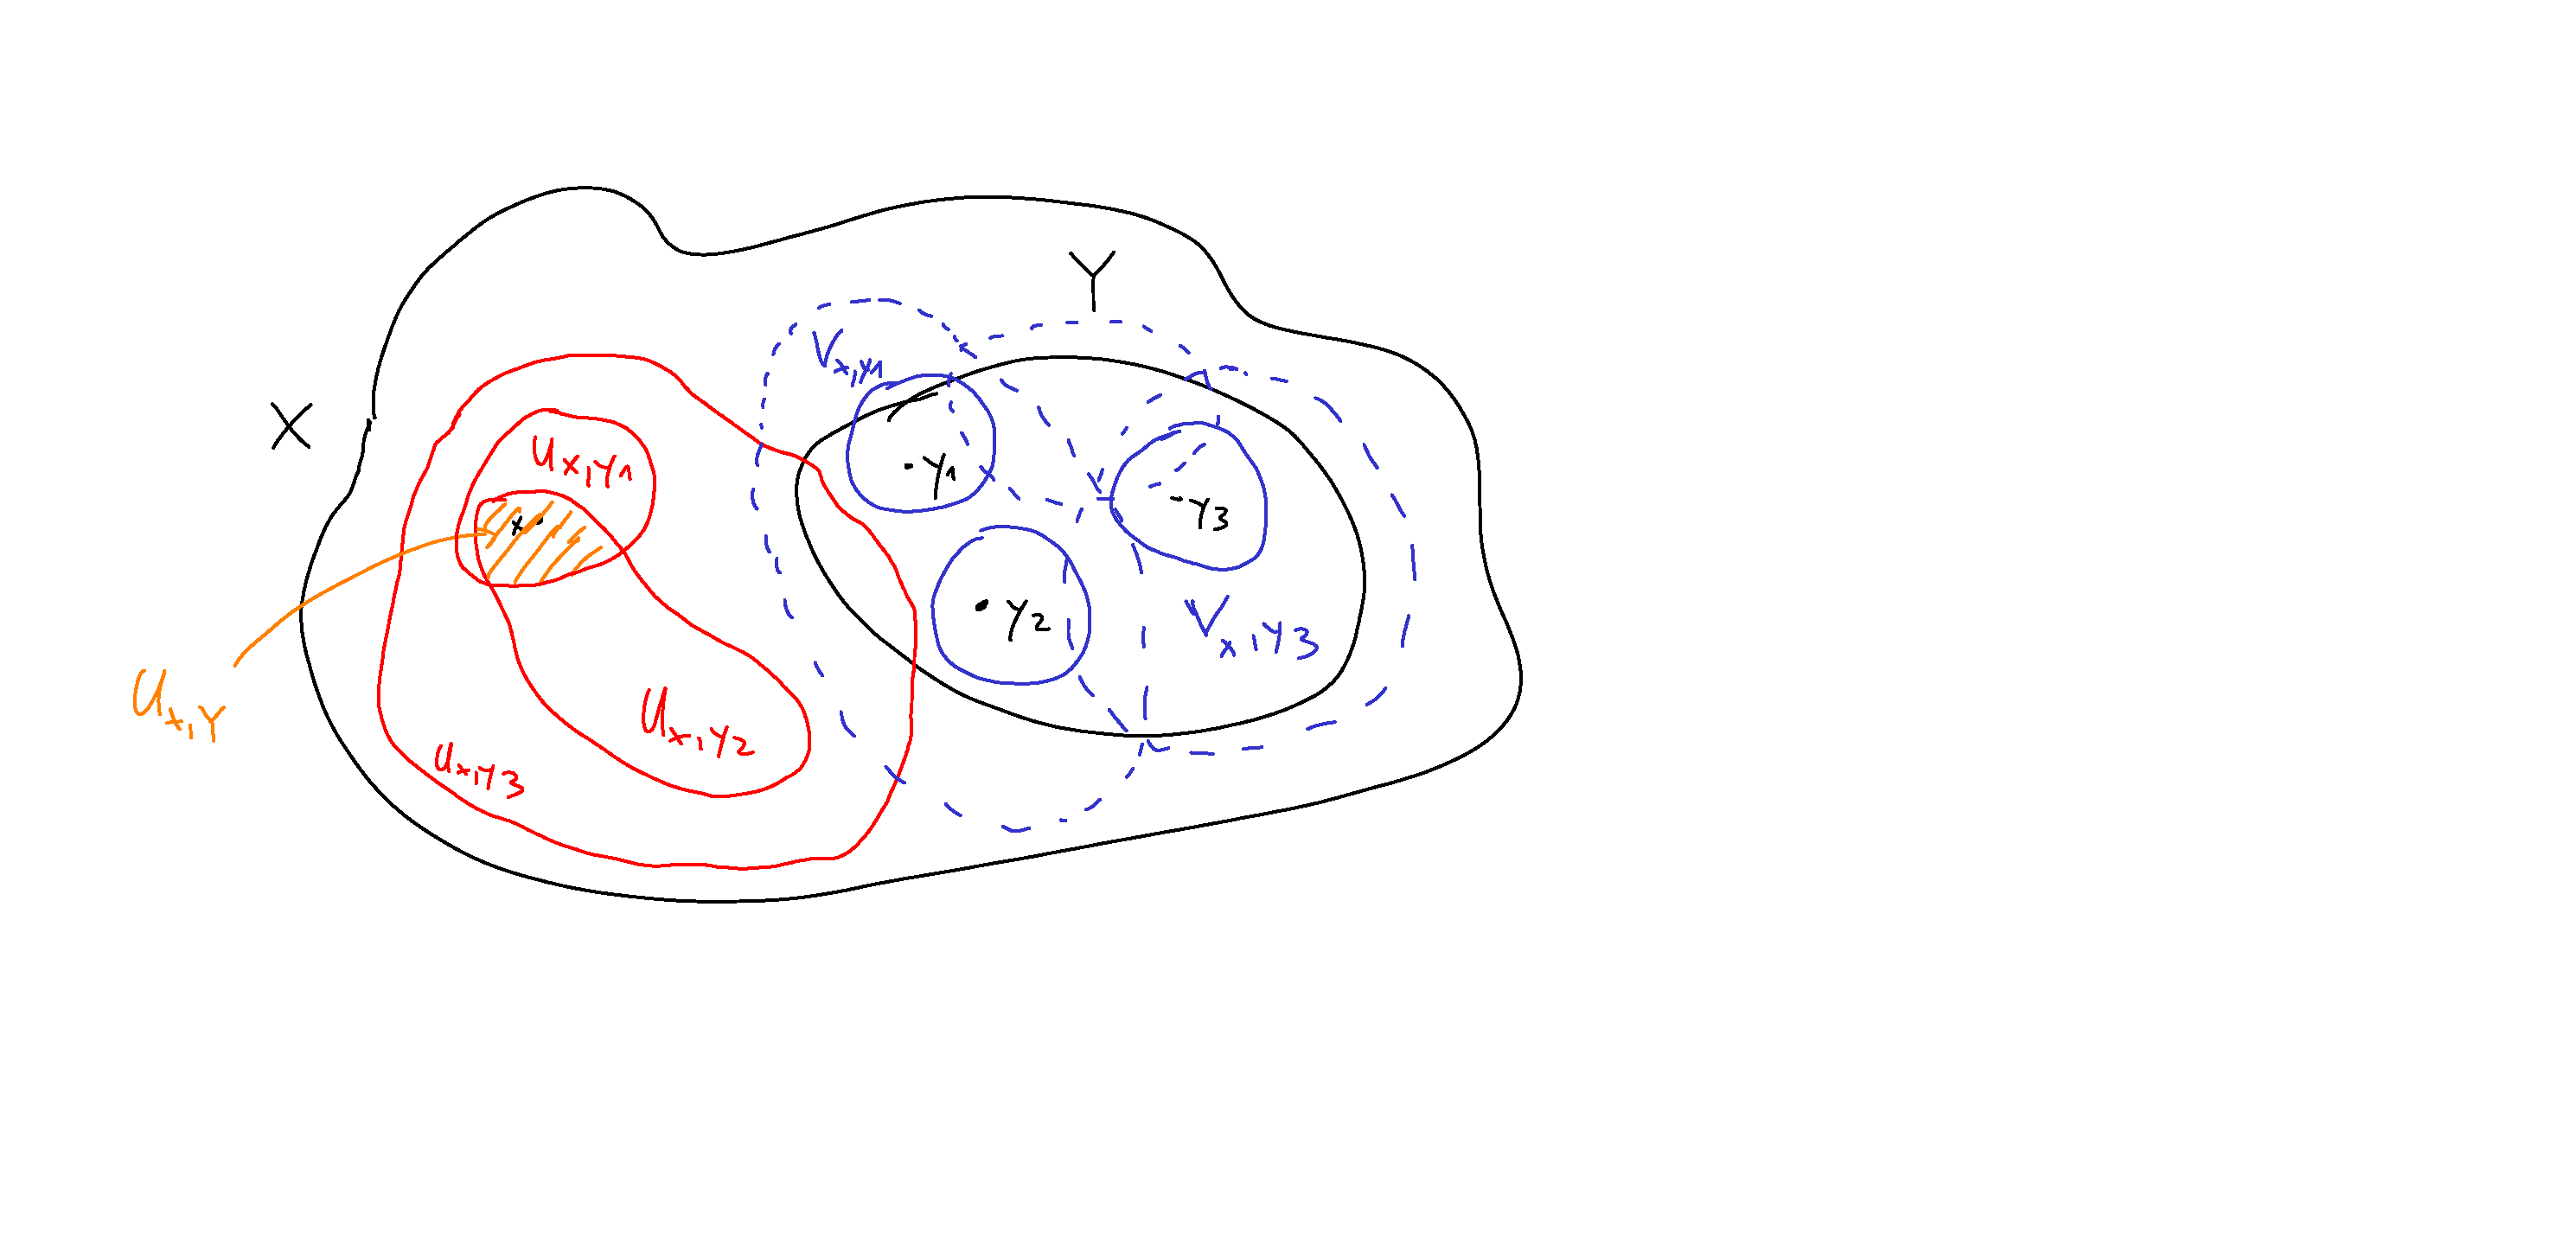
\includegraphics[scale=0.4]{figures/Lemma5.5.pdf}
    \caption{Skizze zum Beweis von Lemma \ref{lm:in-hausdorff-raum-sind-kompakte-mengen-t3}}
\end{figure}
\begin{proof}[Beweis von \autoref{thm:kompakte-menge-in-hausdorff-raum-ist-abgeschlossen}]
    Nach \autoref{lm:in-hausdorff-raum-sind-kompakte-mengen-t3} existieren $\forall x\in X \setminus Y$ ein $U_{x,Y}$ mit $x\in U_{x,Y}$ und $U_{x,Y} \cap Y = \emptyset$. Also ist
    \[
    X \setminus Y = \bigcup_{x\in X \setminus Y} U_{x,Y}
    .\] 
    offen und somit ist $Y$ abgeschlossen.
\end{proof}


\begin{example}['Gegenbeispiel' zu Satz \ref{thm:kompakte-menge-in-hausdorff-raum-ist-abgeschlossen}]
    Sei $G$ die Gerade mit zwei Urpsrüngen: \\
    Betrachte  $\R\cup \left \{0'\right\} $ mit $U$ Umgebung von  $a\in \R$ falls $\exists ε>0$ mit $(a-ε, a+ε)\subset U$ und $U$ Umgebung von  $0'$ und  $U$ Umgebung von  $0'$, falls  $\exists ε>0$ mit $(-ε,0 \cup (0,ε) \subset U$ und $0' \in U$. \\
    Wir können uns gewissermaßen  $0,0'$ gleichberechtigt vorstellen, nur dass die beiden Punkte verschieden sind. \\
    Dann ist  $[-1,1] \subset G$ kompakt (Übung!), aber nicht abegschlossen, da $0' \in G \setminus [-1,1]$ ist, dies aber keine Umgebung von $0'$ ist.
    \begin{figure}[H]
        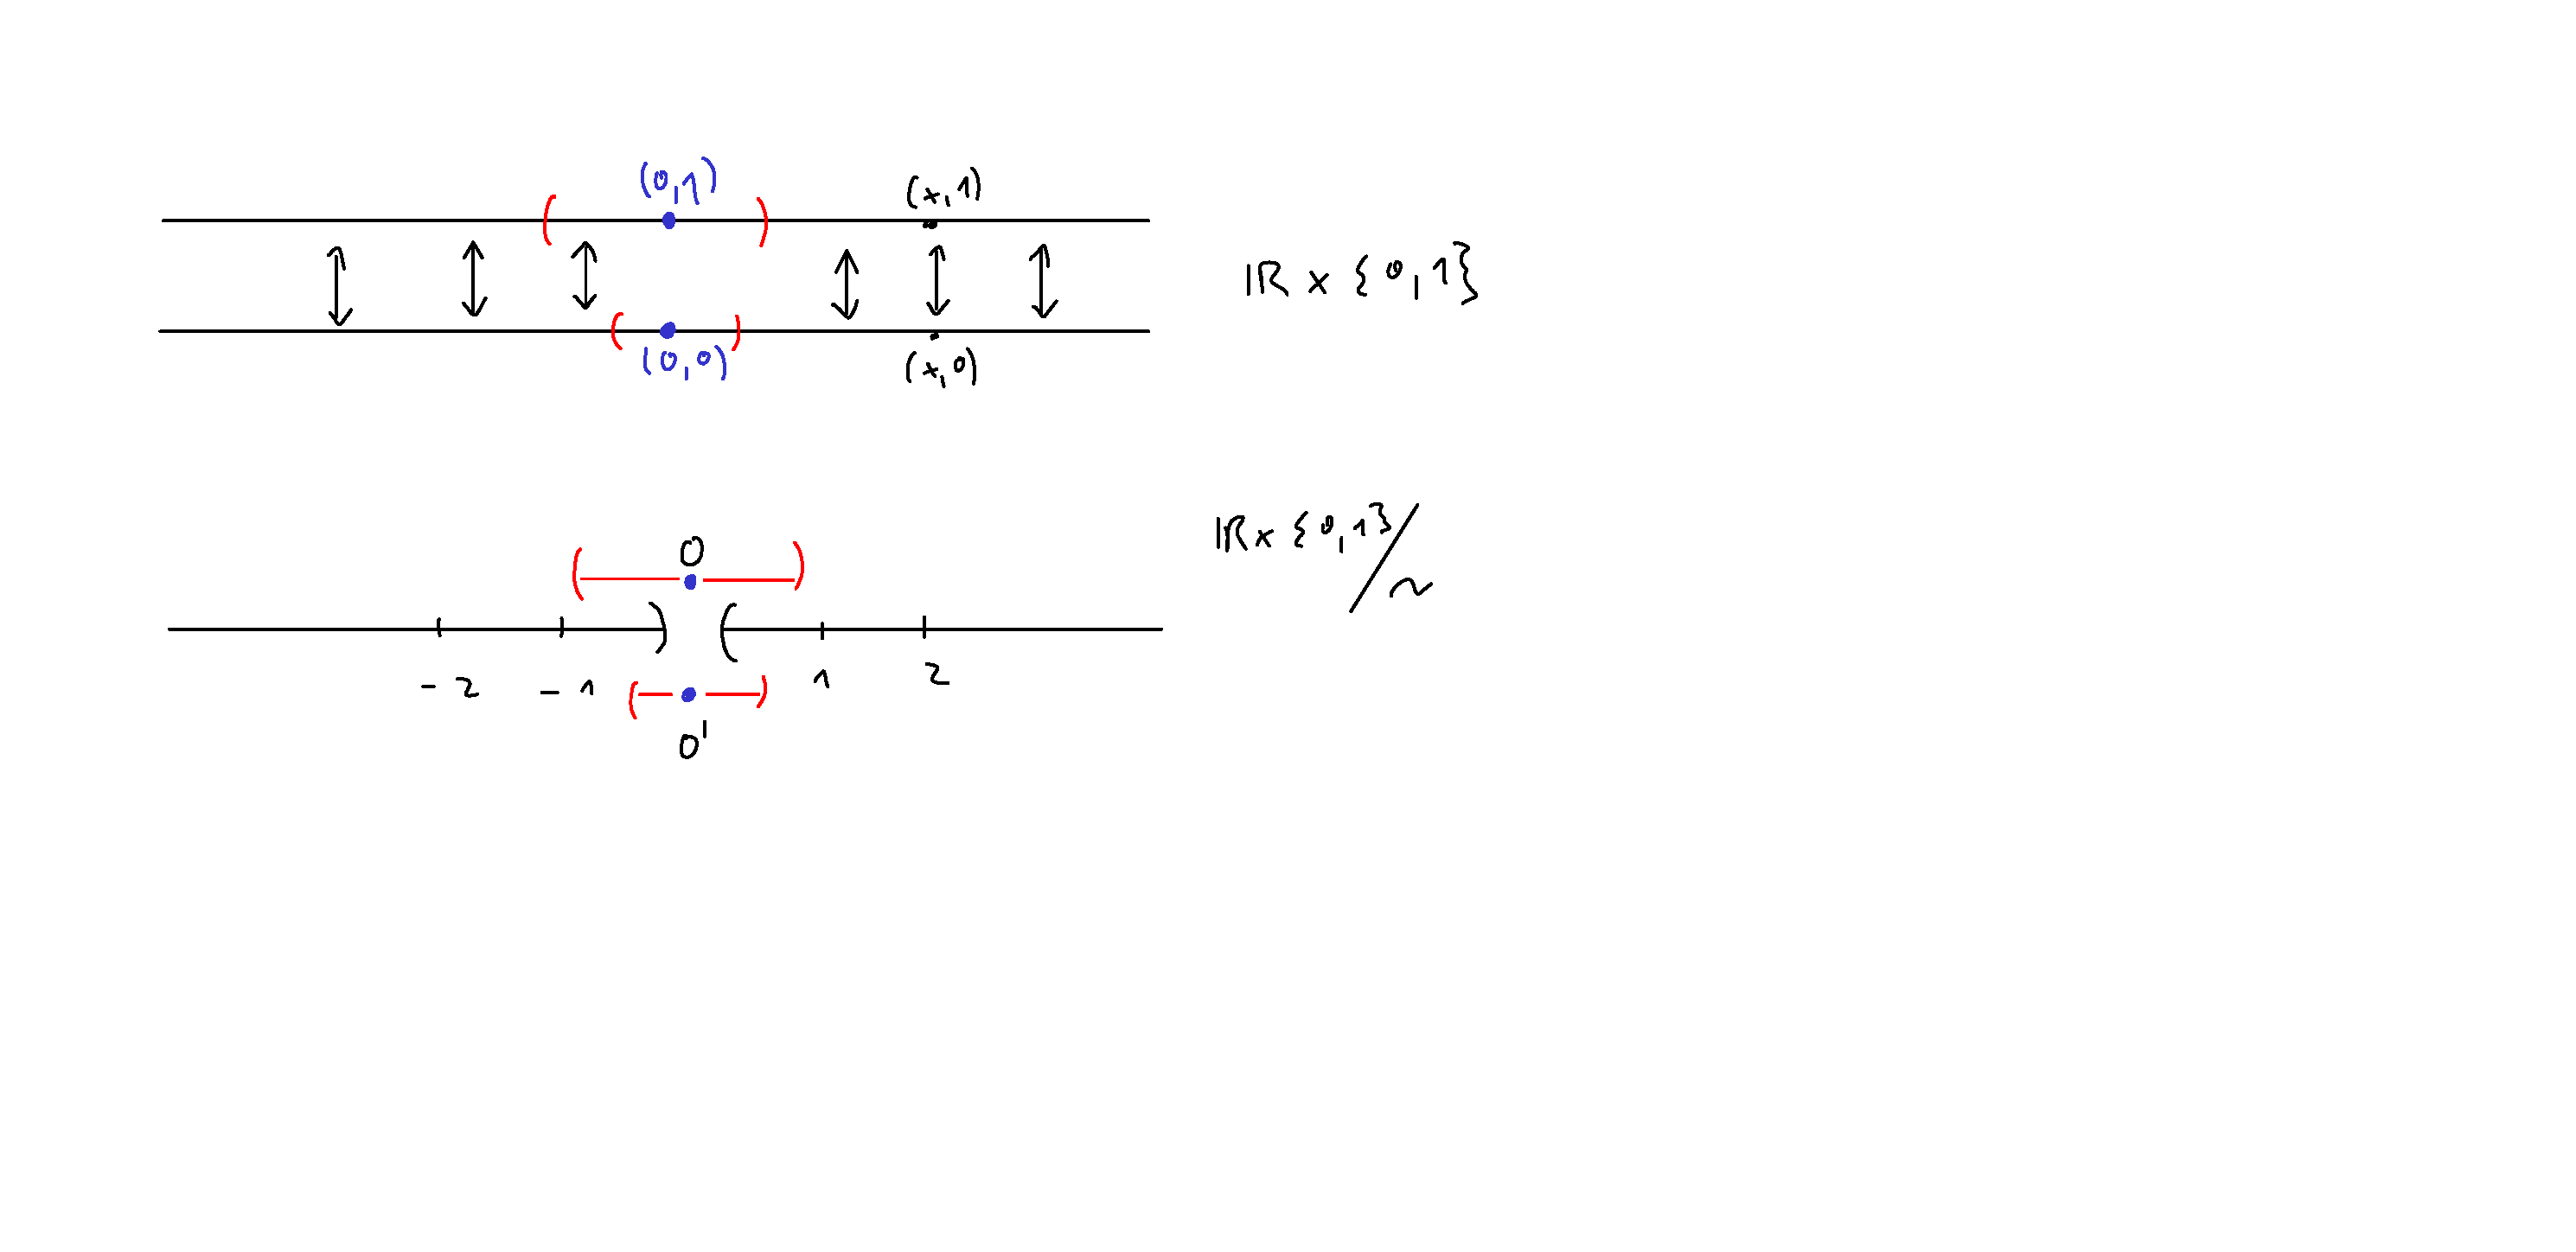
\includegraphics[scale=0.4]{figures/line-with-2-origins.pdf}
    \caption{Gerade mit 2 Ursprüngen}
    \end{figure}
\end{example}

Nun sind wir gewappnet für den
\begin{proof}[Beweis von \autoref{thm:heine-borel} (\nameref{thm:heine-borel})]
    '$2) \implies 1)$'. Sei $X\subset \R^n$ kompakt. Dann ist sie abgeschlossen nach \ref{thm:kompakte-menge-in-hausdorff-raum-ist-abgeschlossen}.
    Zudem ist $X\subset \bigcup_{x\in X} U(x,1)$ eine offene Überdeckung. Da $X$ kompakt finden wir endlich viele  $x_1,\ldots,x_n\in X$ mit
    \[
        X \subset \bigcup_{i=1}^n U(x_i,1)
    .\] 
    Also ist
    \[
        \diam(X) \leq  \max \left \{d(x_i,x_j)\right\} +2 < \infty
    .\] 
    und somit ist $X$ auch beschränkt. \\
    ' $1)\implies 2)$'. Da $X$ beschränkt ist,  $\exists m>0$ mit $X\subset [-m,m]^n\subset \R^n$. Da $X$ abgeschlossen ist, genügt es nach \autoref{thm:abgeschlossene-menge-in-kompaktem-raum-ist-kompakt} zu zeigen, dass  $[-m,m]^n$ kompakt ist. \\
    Wir führen einen Widerspruchsbeweis, nimm also an, dass  $[-m,m]^n$ nicht kompakt ist. Dann existiert eine offene Überdeckung  $\left \{U_i\right\} _{i \in I}$ ohne endliche Teilüberdeckung. \\
    \noindent\begin{minipage}{0.5\textwidth}
    Unterteile $[-m,m]^n$ in  $2^n$ gleich große Unterwürfel (halbiere jede Seite). Mindestens ein Unterwürfel hat keine endliche Teilüberdeckung. Unterteile diesen Würfel weiter und wähle wieder einen Unterwüfel, der keine endliche Teilüberdeckung hat. \\
    Wir erhalten eine Folge von Würfeln
     \[
         [-m,m]^n =     Q_0 \supset Q_1 \supset Q_2 \supset Q_3 \supset \ldots
    .\] 
    die jeweils keine endliche Teilüberdeckung durch $U_i's$ besitzen. \\
    \end{minipage}
    \begin{minipage}{0.5\textwidth}
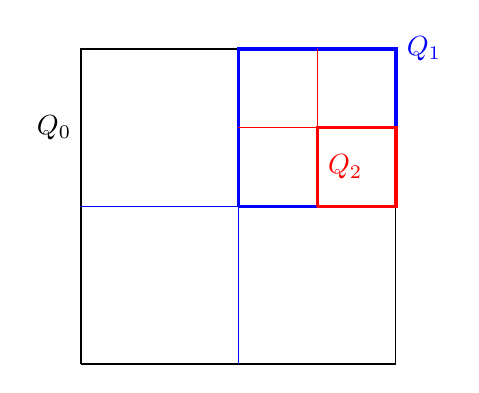
\begin{tikzpicture}
    \draw (-2,-2) -- (-2,2) node[near end, anchor=east]{$Q_0$}-- (2,2) -- (2,-2) -- (-2,-2);
    \draw[blue] (-2,0) -- (2,0);
    \draw[blue] (0,-2) -- (0,2);
    \draw[blue,very thick] (0,0) -- (2,0) -- (2,2) node[anchor=west]{$Q_1$} -- (0,2) -- (0,0) ; 
    \draw[red] (1,0) -- (1,2);
    \draw[red] (0,1) -- (2,1);
    \draw[red, very thick] (1,0) -- (1,1) node[anchor=west, midway]{$Q_2$} -- (2,1) -- (2,0) -- (1,0);
\end{tikzpicture}
    \end{minipage}
    Sei  $x_i \in Q_i$ beliebig. Dann ist $x_i$ eine Cauchy-Folge, also existiert $x = \lim_{i\to \infty} x_i$, und $x\in Q_0$, da $Q_0$ abgeschlossen. \\
    Somit gibt es ein $U_j$ mit  $x\in U_j$, da die $\left \{U_i\right\} _{i \in I}$ eine Überedeckung von $Q_0$ waren. Damit ist auch $U(x,ε) \subset U_j$ für ein $ε>0$. Wähle einen Würfel $x\in Q_k$ mit Kantenlänge $< \frac{ε}{\sqrt{n} }$, dann ist auch $Q_k \subset U(x,ε) \subset U_j$. Das ist aber ein Widerspruch dazu, dass $Q_k$ keine endliche Teilüberdeckung hat, \contra. \\
    Also ist  $Q_0$ kompakt.
\end{proof}



\begin{theorem}[Bilder kompakter Räume]\label{thm:bild-von-kompaktem-raum-ist-kompakt}
    Sei $f: X \to  Y$ stetig und surjektiv und $X$ kompakt. Dann ist auch  $Y$ kompakt. 
\end{theorem}
\begin{proof}
    Sei $\left \{U_i\right\} _{i \in I}$ offene Überdeckung von $Y$. Dann ist
     \[
         \left \{f^{-1}(U_i)\right\} _{i \in I}
    .\] 
    offene Überdeckung von $X$. Da  $X$ kompakt ist, gibt es  $J\subset I$ endlich mit $X = \bigcup_{j\in J} f^{-1}(U_j)$. Dann ist 
    \[
        Y = f(X) = \bigcup_{j\in J} f(f^{-1}(U_j)) = \bigcup_{j\in J} U_j
    .\] 
    Also existiert eine endliche Teilüberdeckung von $Y$.
\end{proof}
\begin{corollary}\label{cor:stetige-abbildung-von-kompaktem-raum-in-hausdorff-raum-ist-abgeschlossen}
    Sei $f: X \to  Y$ stetig, $X$ kompakt und  $Y$ Hausdorff. Dann ist  $f$ abgeschlossen, d.h. $\forall A\subset X$ abgeschlossen ist $f(A) \subset Y$ abgeschlossen.
\end{corollary}
\begin{proof}
    Sei $A\subset X$ abgeschlossen. Dann ist $A$ kompakt nach \autoref{thm:kompakte-menge-in-hausdorff-raum-ist-abgeschlossen}, also ist  $f(A)$ kompakt nach \autoref{thm:bild-von-kompaktem-raum-ist-kompakt} (weil $f: X \to f(A)\subset Y$ surjektiv ist). Damit ist dann $f(A)$ abegschlossen nach \autoref{thm:kompakte-menge-in-hausdorff-raum-ist-abgeschlossen}. \\
    Also sind Bilder abgeschlossener Mengen abgeschlossen.
\end{proof}

\begin{corollary}[Homöomorphismen]\label{cor:stetige-bijektion-von-kompaktem-raum-in-hausdorff-raum-ist-homöomorphismus}
    Ist $f: X \to  Y$ stetig und bijektiv, $X$ kompakt und  $Y$ Hausdorff, dann ist  $f$ ein Homöomorphismus.
\end{corollary}

\begin{proof}
    Wir müssen zeigen, dass die Umkehrabbildung stetig ist. Dafür reicht es zu zeigen, dass $\forall A\subset X$ abgeschlossen auch $f(A) = (f^{-1})^{-1}(A)$ abgeschlossen ist. Das gilt aber genau nach vorherigem \autoref{cor:stetige-abbildung-von-kompaktem-raum-in-hausdorff-raum-ist-abgeschlossen}
\end{proof}
\begin{corollary}\label{cor:abbildung-von-kompaktem-raum-in-hausdorff-raum-ist-quotientenabbildung}
    Sei $f: X \to  Y$ stetig und surjektiv, $X$ kompakt und  $Y$ Hausdorffsch. Dann trägt  $Y$ die Quotiententopologie, d.h.  $U\subset Y$ offen genau dann, wenn $f^{-1}(U) \subset X$ offen.
\end{corollary}

\begin{proof}
    '$\implies$' folgt wegen Stetigkeit. \\
    '$\impliedby$' Ist $f^{-1}(U) \subset X$ offen, dann ist $f^{-1}(Y \setminus U ) = X \setminus f^{-1}(U)$ abgeschlossen in $X$, also folgt aus dem \autoref{cor:stetige-abbildung-von-kompaktem-raum-in-hausdorff-raum-ist-abgeschlossen}
     \[
         Y \setminus U \stackrel{\text{surj.}}{=}   f\left( \underbrace{f^{-1}\left( Y \setminus U \right)}_{\text{abgeschlossen}}  \right) 
    .\] 
    abgeschlossen ist, also ist $U\subset Y$ offen.
\end{proof}
Kommen wir nun zum
\begin{proof}[Beweis von \autoref{thm:kreis-ist-quotientenraum-von-einheitsintervall}]
    Schon gezeigt:
        \begin{equation*}
        \begin{array}{c c l} 
            [0,1] & \longrightarrow & S_1 \\
        t & \longmapsto &  2^{2\pi it}
        \end{array}
    \end{equation*}
    ist stetig und surjektiv und faktorisiert über
    \[
        [0,1] /\left \{0,1\right\}  \to  S^1
    .\] 
    mit $f$ stetig und bijektiv. Wir wissen nun:  $S^1$ ist Hausdorffsch und  $[0,1]$ ist kompakt. Nach \autoref{thm:bild-von-kompaktem-raum-ist-kompakt} ist auch  $[0,1] /\left \{0,1\right\} $ kompakt, also ist $f$ ein Homöomorphismus nach \autoref{cor:stetige-bijektion-von-kompaktem-raum-in-hausdorff-raum-ist-homöomorphismus}
\end{proof}


\begin{theorem}\label{thm:kompakter-hausdorff-raum-ist-normal}
    Jeder kompakte Hausdorff-Raum ist normal.
\end{theorem}
\begin{proof}
    Seien $A,B\subset X$ abgeschlossen und disjunkt. Da $X$ kompakt ist, sind  $A,B$ kompakt. Nach Lemma 5.5 existieren  $\forall a\in A$ offene Mengen $U_a, V_a$ mit $a\in U_a, B\subset V_a$ und $U_a \cap V_a = \emptyset$. Dann ist
    \[
    A \subset \bigcup_{a\in A} U_a
    .\] 
    Also existieren $a_1,\ldots,a_n\in A$ mit
    \[
    A\subset \bigcup_{i=1}^n U_{a_i}
    .\] 
    wegen $A$ kompakt. Setze nun
    \[
    U_A := \bigcup_{i=1}^n U_{a_i}\supset A \qquad U_B := \bigcap_{i=1}^n V_{a_i}\supset B
    .\] 
$\forall i$ ist 
\[
    U_{a_i} \cap U_B \subset U_{a_i} \cap V_{a_i} = \emptyset
.\] 
und daraus folgt, dass
\[
U_A \cap U_B = \emptyset
.\] 
\end{proof}

\begin{theorem}[Quotientenräume von Hausdorffräumen]\label{thm:quotientenraum-von-hausdorffraum-ist-hausdorff-gdw-projektion-abgeschlossen}
    Sei $X$ kompakt und Hausdorffsch, $q: X \to  Z$ surjektiv, wobei  $Z$ die Quotiententopologie trage. Dann sind äquivalent: 
    \begin{enumerate}[1)]
        \item $Z$ ist Hausdorffsch
        \item  $q$ ist abgeschlossen
    \end{enumerate}
\end{theorem}
\begin{proof}
    Die Richtung '$1) \implies 2)$' ist genau \autoref{cor:stetige-abbildung-von-kompaktem-raum-in-hausdorff-raum-ist-abgeschlossen} \\
    '$2)\implies_1)$': Jedes $z\in Z$ hat ein Urbild $x\in X$ unter $q$. Es ist  $\left \{x\right\} \subset X$ abgeschlossen, da $X$ hausdorffsch. Wegen  $q$ abgeschlossen folgt nun, dass auch
    \[
        \left \{z\right\}  = q(\left \{x\right\} )
    .\] 
    abgeschlossen ist. \\
    Wir nennen Teilmenge $W\subset X$ heißt \vocab[Menge!saturiert]{saturiert}, falls $W = q^{-1}(q(W))$ (insbesondere sind alle Urbilder saturiert, und $\iff  \forall x\in X \setminus W : g(x) \in Z \setminus g(W)$). \\
\begin{remark}
    Sei $U\subset X$ offen und saturiert, dann ist $q(U)$ offen. Hierzu schreibe
    \[
        U = q^{-1}(q(U)) \implies q(U) \text{ offen}
    .\] 
\end{remark}
Seien $y\neq z\in Z$. Dann sind $\left \{y\right\} ,\left \{z\right\} $ abgeschlossen und disjunkt. Dann sind auch
\[
    A = q^{-1}(y) \qquad B = q^{-1}(z)
.\] 
abgeschlossen und disjunkt (in  $X$). Nach Annahme ist  $X$ kompakt und Hausdorff, also normal nach Satz \ref{thm:kompakter-hausdorff-raum-ist-normal}. Also existieren  $U_1,U_2\subset X$ offen mit $A\subset U_1,B\subset U_2$ und $U_1 \cap U_2 = \emptyset$. Setze
\[
    V_1 := X \setminus q^{-1}(q(X\setminus U_1)) \qquad V_2 := X \setminus q^{-1}(q(X\setminus U_2))
.\] 
\begin{claim}
    Es sind $V_1,V_2$ offen, disjunkt und saturiert und $A\subset V_1$ sowie $B\subset V_2$.
\end{claim}
\begin{subproof}
    Nächstes Mal.
\end{subproof}
Es folgt, dass $q(V_1),q(V_2)$ offen in $Z$ sind. Weiter ist  $y\in q(A)\subset q(V_1)$ und $z\in q(B) \subset q(V_2)$. Da $V_1,V_2$ disjunkt und saturiert, sind auch $q(V_1),q(V_2)$ disjunkt und wir sind fertig.
\end{proof}

    \lecture{5}{Di 27 Apr 2021 12:16}{}
\begin{proof}[Beweis der Behauptung]
    Es ist klar, dass $V_1, V_2$ offen sind. Für Disjunktheit sehen wir mit
    \[
        X \setminus U_i \subset  q^{-1}(q(X\setminus U_i))
    .\] 
    dass $U_i \supset X \setminus q^{-1}(q(X\setminus U_i)) = V_i$ 
    Für Saturiertheit genügt es zu sehen, dass $g^{-1}(C)$ saturiert ist für alle $C\subset Z$, da
    \[
        q^{-1}(q(q^{-1}(C))) = q^{-1}(C)
    .\] 
    weil $q$ surjektiv ist. Wegen
     \[
         A\subset U_1 \implies X \setminus A \supset X \setminus U_1 \implies q(X\setminus A) \supset q(X\setminus U_1) \implies \underbrace{q^{-1}(q(X\setminus A))}_{=X\setminus A} = q^{-1}q(X\setminus U_1)
    .\]
    Komplementbildung liefert unser gewünschtes Eregbnis.
\end{proof}


\begin{example}
    $\R \mathbb{P}^n$ ist Hausdorffsch. 
    \begin{proof}
        Es ist $\R \mathbb{P}^n \cong S^n / x \sim  - x$. Sei
        \[
        q : S^n \to  S^n / x\sim -x
        .\] 
    \end{proof}
    die Projektion. Da $S^n$ kompakt und Hausdorffsch ist, ist  $\R \mathbb{P}^n$ Hausdorffsch genau dann, wenn $q$ abgeschlossen ist. Ist  $A\subset S^n$, so ist $q^{-1}(Q(A)) = A \cup -A$. \\
Da $-: S^n \to  S^n$ ein Homöomorphismus ist, ist $-A$ abgeschlossen, wenn  $A$ abgeschlossen ist. Dann ist auch  $A \cup -A$ abgeschlossen.
\end{example}
\begin{corollary}
    Sei $\sim $ auf $D^n = \left \{x \in \R^n \mid  \lVert x \rVert \leq 1\right\} $ erzeugt durch $x \sim -x$ für alle $x\in S^{n-1}\subset D^n$. Dann ist
    \[
    D^n / \sim  \cong \R \mathbb{P}^n
    .\] 
    Insbesondere ist 
    \[
        \R\mathbb{P}^1 \cong D^1 / \left \{-1,1\right\} \cong [0,1] / \left \{0,1\right\}  \cong S^1
    \]
    \label{cor:}
\end{corollary}
\begin{proof}
    Betrachte die stetige Abbildung
        \begin{equation*}
        f: \left| \begin{array}{c c l} 
        D^n & \longrightarrow & S^n \\
        x& \longmapsto &  (x,\sqrt{1-\lVert x \rVert ^2}) 
        \end{array} \right.
    \end{equation*}

    \todo{        Skizze einfügen für 'ausbeulen' der Abbildung.}
    Wir erhalten das Diagramm
    \begin{figure}[h]
        \centering
    \begin{tikzcd}
        D^n \ar{r} \ar{d} & S^n \ar{d} \\
    D^n / \sim \ar[dashed,swap]{r}{\overline{f}} & S^n / (x\sim -x) \cong \R\mathbb{P}^n
    \end{tikzcd}
    \end{figure}
    Wir sehen leicht, dass $\overline{f}$ bijektiv ist. Da $D^n$ kompakt, ist auch  $D^n / \sim $ kompakt, und $\R\mathbb{P}^n$ ist Hausdorffsch, also handelt es sich um einen Homöomorphismus (mit \ref{cor:compact-to-hausdorff-is-homeomorphism})
\end{proof}

\begin{corollary}
    Sei $X$ kompakt und Hausdorffsch und  $A\subset X$. Dann sind äquivalent
    \begin{enumerate}[1)]
        \item $X / A$ ist Hausdorffsch
        \item  $A$ ist abgeschlossen.
    \end{enumerate}
\end{corollary}
\begin{proof}
    '$1)\implies_2)$'. Ist $X // A$ Hausdorffsch, so ist die einpunktige Menge $\left \{A\right\} $ abgeschlossen (nach \ref{thm:point-in-hausdorff-space-is-closed}). Also ist $q^{-1}(A) = A$ abgeschlossen. \\
    '$2)\implies 1)$' Nach \ref{thm:quotient-space-of-compact-hausdorff-space} genügt es zu zeigen, dass $q: X \to  X / A$ abgeschlossen ist. Für $B\subset X$ abgeschlossen ist
    \[
        q^{-1}(q(B)) = \begin{cases}
            B & \text{falls } B\cap A = \emptyset \\
            B \cup A & \text{falls }B \cap  A \neq  \emptyset
        \end{cases}
    .\] 
    abgeschlossen, weil $A$ abgeschlossen ist. 
\end{proof}


\begin{example}
    \begin{enumerate}[a)]
        \item
Es ist $D^n / S^{n-1}$   Hausdorffsch. Alternativ können wir auch sehen, dass $D^n / S^{n-1} \cong S^n$ ist. Hierzu betrachte die Projektion:
    \begin{equation*}
    \begin{array}{c c l} 
    D^n & \longrightarrow & S^n \\
    x & \longmapsto &  \begin{cases}
        (2x, \sqrt{1-\lVert 2x \rVert ^2} & 0 \leq  \lVert x \rVert \leq \frac{1}{2}  \\
        \left( \frac{2-2\lVert x \rVert }{\lVert x \rVert }\cdot x, - \sqrt{1-(2-2\lVert x \rVert )^2}  \right) & \frac{1}{2} \leq  \lVert x \rVert  \leq 1
    \end{cases}
    \end{array}
\end{equation*}
Diese ist stetig, denn falls $\lVert x \rVert =\frac{1}{2}$ ist
\item Wir erhalten nun eine Abbildung 
\[
\frac{2-2\lVert x \rVert }{\lVert x \rVert } = \frac{2-1}{\frac{1}{2}} = 2
.\] 
und
\[
    \sqrt{1-\lVert 2x \rVert ^2} = \sqrt{1-1} =0 = - \sqrt{0} = -\sqrt{1-(2-2\lVert x \rVert )^2}  
.\] 
Ist $\lVert x \rVert =1$, so ist
 \[
\frac{2-2\lVert x \rVert }{\lVert x \rVert } = 0
.\] 
und somit ist $f(x) = (0,-1) \in \R^n \times \R$. Also faktorisiert $f$ über  $\overline{f} : D^n / S^{n-1} \to  S^n$. Wir sehen wieder leicht, dass $\overline{f}$ stetige Bijektion ist. Da $D^n / S^{n-1}$ kompakt und $S^n$ Hausdorffsch, folgt wieder, dass  $\overline{f}$ ein Homöomorphismus ist. \\
    \begin{tikzcd}
        S^n \ar{r}{q} & S^n / (x\sim -x) \cong \R\mathbb{P}^n \cong D^n / (x\sim -x) \ar{r} &  D^n / S^{n-1} \cong S^n
    \end{tikzcd}
    \end{enumerate}
\end{example}
\todo{Abbildung skizzieren}

\def\Base{\mathcal{S}} %temporary
\section{Basen und Subbasen}
\begin{definition}
    Sei $(X, \mathcal{O})$ ein topologischer Raum. Sei $\Base \subset \mathcal{O}$ eine Menge offener Mengen. Dann heißt $\Base$
    \begin{description}
        \item[\vocab{Basis}], falls $\forall U\subset \mathcal{O}$ existiert $S_i \in \Base$ mit $U = \bigcup_{i\in I} S_i$ 
        \item[\vocab{Subbasis}], falls $\forall U\in \mathcal{O}$ existieren $I, K_i$ endlich sowie  $S_k \in  \Base$ mit 
            \[
            U = \bigcup_{i\in I} \bigcap_{k\in K_i} S_k 
            .\] 
    \end{description}
\end{definition}
\begin{remark}
Ist     $\Base$ eine Basis, so ist $\Base$ eine Subbasis.
\end{remark}
\begin{example}
    Ist $(X,d)$ ein metrischer Raum, so ist
     \[
         \Base = \left \{U(x,ε) \mid  x\in X, ε>0\right\} 
    .\] 
    eine Basis der Topologie.
\end{example}
\begin{theorem}
    Sei $X$ eine Menge,  $\Base \subset \mathcal{P}(X)$ eine Menge von Teilmengen. Dann existiert genau eine Topologie auf  $X$, für die  $\Base$ eine Subbasis ist, nämlich:
     \[
    \mathcal{O} = \left \{U\subset X \mid  U = \bigcup_{i \in  I} \bigcap_{k\in K_i} S_k \text{ mit } \abs{K_i}<\infty, S_k \in  \Base  \right\} 
    .\] 
\end{theorem}
\begin{proof}
    Übung.
\end{proof}
\begin{notation}
    Wir nennen $\mathcal{O}$ die \vocab{von $\Base$ erzeugte Topologie}.
\end{notation}
\begin{lemma}
    Sei $f: X \to  Y$ eine Abbildung zwischen topologischen Räumen, $\Base$ eine Subbasis von $Y$. Dann sind äquivalent:
    \begin{enumerate}[1)]
        \item $f$ ist stetig
        \item  $f^{-1}(S)$ ist offen für alle $S\in \Base$
    \end{enumerate}
\end{lemma}
\begin{proof}
    '$1) \implies 2)$' ist klar, da Subbasiselemente offen sind. \\
    '$2) \implies 1)$'. Sei $U \subset Y$ offen, dann $\exists K_i$ endlich und $S_k \in \Base$ mit
    \[
    U = \bigcup_{i \in  I} \bigcap_{k\in K_i} S_k
    .\] 
    Dann ist aber genau
    \[
        f^{-1}(U) = \bigcup_{i \in  I} \bigcap_{k\in K_i} \underbrace{f^{-1}(S_k)}_{\text{offen}} 
    .\] 
    offen, weil endliche Schnitte und beliebige Vereinigung offener Mengen offen sind. Also ist $f$ stetig.
\end{proof}

\begin{theorem}
    Eine Subbasis $\Base$ von  $(X, \mathcal{O})$ ist eine Basis genau dann, wenn
    \[
    \forall S_1, S_2 \in \Base \;\exists S_i \in \Base \colon S_1 \cap S_2 = \bigcup_{i \in I} S_i
    .\] 
\end{theorem}
\begin{proof}
'$\implies$'    Da $S_1,S_2 \in \Base$ sind diese offen. Dann ist auch $S_1\cap S_2$ offen. Ist $\Base$ Basis, dann gibt es also  $S_i \in  \Base$ mit 
\[
S_1 \cap  S_2 = \bigcup_{i \in  I} S_i
.\] 
'$\impliedby$' Angenommen, $U\subset X$ ist offen und von der Form
\[
    U = \bigcup_{i \in  I} \left( \bigcap_{k\in K_i} S_k \right) 
.\] 
mit $K_i$ endlich und  $S_k \in  \Base$. Nach Annahme ist
\[
\bigcap_{k\in K_i} = \bigcup_{j\in J_i} S_j  
.\] 
und damit ist
\[
U = \bigcup_{i\in I} \bigcup_{j\in J_i} S_j  
.\] 
\end{proof}
\begin{remark}
    Nach Annahme ist eigentlich erstmal der Schnitt von 2 Mengen die Vereinigung von $S_i$. Allerdings kann man dies per Induktion leicht auf  $n$ Teilmengen verallgemeinern, wenn wir
     \[
         \bigcap_{k=1}^n S_k = S_1 \cap  \bigcap_{k=2}^{n} S_k = S_1 \cap \bigcup_{i\in I} S_i = \bigcap_{i\in I} (S_i \cap S_k) = \bigcup_{i\in I} \bigcup_{j\in J_i} S_j  
    .\]
    für geeignete $S_i, S_j\in \Base$ schreiben.
\end{remark}
\begin{theorem}
    \label{thm:alexander}
    Sei $X$ ein topologischer Raum und  $\Base$ eine Subbasis. Dann ist  $X$ kompakt genau dann, wenn jede Überdeckung durch Elemente aus  $\Base$ eine endliche Teilüberdeckung besitzt.
\end{theorem}
\begin{proof}
    '$\implies$' ist klar. \\
    '$\impliedby$' Angenommen, $X$ ist nicht kompakt, dann betrachte die Menge
     \[
    \mathcal{C} := \left \{U \mid  U \text{ offene Überdeckung \underline{ohne} endliche Teilüberdeckung}\right\} \neq \emptyset
    .\] 
    Es ist $\mathcal{C}$ partiell geordnet, indem wir $U\leq U'$ für $U\subset U'$ setzen. \\
    Ist $U_1\subset U_2\subset \ldots$ eine Kette, so ist $\bigcup_{U_i}\in \mathcal{C}$, denn
    \begin{itemize}
        \item Offenbar ist $\bigcup_{i \in  I} U_i$ eine offene Überdeckung.
        \item Hat $\bigcup_{i \in  I} U_i$ eine endliche Teilüberdeckung, so ist diese schon in einem $U_i$ enthalten, und damit enthielte auch dieses  $U_i$ bereits eine endliche Teilüberedckung \contra
    \end{itemize}
Wir können also das Lemma von Zorn anwenden, und somit existiert ein maximales Elment $U\in \mathcal{C}$.
\begin{claim}
    Ist $V\subset X$ offen und  $V\not\in U$, so hat $U\cup \left \{V\right\} $ eine endliche Teilüberdeckung
\end{claim}
\begin{subproof}
    Sonst wäre $U \cup \left \{V\right\} \in \mathcal{C}$ und somit wäre $U$ nicht maximal
\end{subproof}
\begin{claim}
    $U \cap \Base$ ist keine Überdeckung
\end{claim}
\begin{subproof}
    Sonst hätte $U$ eine endliche Teilüberedckung nach Annahme.
\end{subproof}
Wegen Behauptung 2 existiert $x\in X$, der nicht von $U \cap \Base$ überdeckt wird. Sei $W\in U$ mit $x\in W$. Da $W$ offen ist, folgt
 \[
W = \bigcup_{i \in  I} \bigcap_{k\in K_i} S_k
.\] 
mit $K_i$ endlich und  $S_k \in \Base$. Dann existieren also $S_1,\ldots,S_n$ mit 
\[
x \in  \bigcap_{i=1}^n S_i \subset W 
.\] 
Da $x$ nicht von  $U \cap \Base$ überdeckt wird, ist $S_i \not\in U$. Aus der ersten Behauptung wissen wir nun aber, dass es $U_1^i, \ldots, u_{n_i}^i \in U$ mit
\[
\left \{U_j ^i\right\} _{j=1}^n \cup \left \{S_i\right\}  \quad \text{ ist Überdeckung von } X
.\] 
Sei nun 
\[
\hat{U} := \left \{U_j ^i \mid  1\leq i\leq n, 1\leq j\leq n_i\right\} \subset U
.\] 
Für alle $i$ gilt also
 \[
X \subset \bigcup_{V\in \hat{U}} V \cup S_i 
.\] 
Also folgt
\[
X \setminus \bigcup_{V\in \hat{U}} V \subset S_i 
.\] 
und damit ist auch
\[
X\setminus \bigcup_{V\in \hat{U}} V \subset S_1 \cap \ldots \cap S_n \subset W \in U 
.\] 
Also ist $\hat{U}\cup \left \{W\right\} $ eine endliche Teilüberdeckung von $U$, \contra.
\end{proof}

    % end lectures
\end{document}
